\documentclass[12pt,a4paper]{article}
\usepackage{amsfonts, amssymb, amsmath}
\usepackage{fullpage}
\usepackage{parskip} % skip a line instead of indenting
\usepackage{amsthm}
\usepackage{xcolor}
\usepackage{tikz}

\newtheorem*{rem}{Remark}

\title{Vector Spaces and Subspaces}
\author{R4 Cheng}
\date{\today}

\newcommand{\Remark}[1]{
  \begin{rem}
    \color{cyan}
    #1
  \end{rem}
}

\begin{document}
\maketitle

$\mathbb{R}^n = $ all (column) vectors with n (real) components. \\
$= \{ (v_1, v_2, \cdots, v_n): v_i \in \mathbb{R}, i = 1, 2, \cdots, n \}$

\[
\begin{bmatrix}
  4 \\
  \pi \\
\end{bmatrix} \in \mathbb{R}^2,
\quad
(1, 1, 0, 1, 1) \in \mathbb{R}^5
\]
\[
\begin{tikzpicture}
  % Draw x-axis
  \draw[->] (-2, 0) -- (2, 0) node[right] {$x$};
  % Draw y-axis
  \draw[->] (0, -2) -- (0, 2) node[above] {$y$};
  
  % Draw vector v
  \draw[->, red] (0, 0) -- (1, 1) node[midway, below right] {$\mathbf{v}$};
  \draw[->, pink] (0, 0) -- (3, 3) node[midway, above right] {$\mathbf{3v}$};
  
  % Draw vector w
  \draw[->, blue] (0, 0) -- (1, 2) node[midway, above left] {$\mathbf{w}$};
  
  % Draw vector v + vector w
  \draw[->, purple] (0, 0) -- (2, 3) node[above right] {$\mathbf{v} + \mathbf{w}$};
\end{tikzpicture}
\]

\subsection*{Vector Space $V$}

$V$: a set of vectors
\begin{enumerate}
  \item Two operations:
  \begin{itemize}
    \item vector addition: $\underline{v}, \underline{w} \in V \Rightarrow \underline{v} + \underline{w} \in V$
    \item scalar multiplication: $c \underline{v} \in V$
  \end{itemize}
  \item Eight rules:
  \begin{enumerate}
    \item $\underline{v} + \underline{w} = \underline{w} + \underline{v}$ (commutative)
    \item $(\underline{v} + \underline{w}) + \underline{z} = \underline{v} + (\underline{w} + \underline{z})$ (associative)
    \item There is a unique "zero vector" \underline{0} such that $\underline{v} + \underline{0} = \underline{v}$ for all $\underline{v} \in V$
    \item For each $\underline{v}$, there is a unique vector $-\underline{v}$ such that $\underline{v} + (-\underline{v}) = \underline{0}$
    \item $1 \times \underline{v} = \underline{v}$
    \item $(c_1c_2)\underline{v} = c_1(c_2\underline{v})$
    \item $c(\underline{v} + \underline{w}) = c\underline{v} + c\underline{w}$
    \item $(c_1 + c_2)\underline{v} = c_1\underline{v} + c_2\underline{v}$
  \end{enumerate}
\end{enumerate}

$\Rightarrow 0 \times \underline{v}  = \underline{0}$  (not 0) \\
$\Rightarrow (-1)\underline{v} = -\underline{v}$

Example:

\begin{itemize}
  \item $\mathbb{R}^n$ is a vector space
  \item $M =$ \{all real $2 \times 2$ matrices\} is a vector space
  \item $F =$ \{all real functions $f(x)$ \} is a vector space
  \item $z = \{ \underline{0} \}$ is a vector space
\end{itemize}

\subsection*{Subspaces}

\textbf{Def.} A subset W of a vector space V is a \underline{subspaces} if W itself is a vector space.

\textbf{Claim} Every subspace contains the zero vector.

\textbf{Proof} TODO

Example:

1. 

$U = \{(x, y): x \geq 0, y \geq 0\}$, is $U$ a subspace?
$
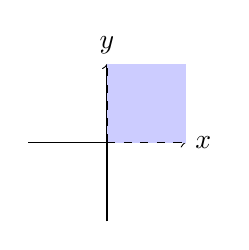
\begin{tikzpicture}
  % Draw x-axis
  \draw[->] (-1, 0) -- (1, 0) node[right] {$x$};
  % Draw y-axis
  \draw[->] (0, -1) -- (0, 1) node[above] {$y$};

  % Shade the first quadrant
  \fill[color=blue!20] (0,0) rectangle (1,1);
    
  % Draw dashed lines along the boundaries
  \draw[dashed] (0,0) -- (1,0);
  \draw[dashed] (0,0) -- (0,1);
\end{tikzpicture}
$

No, since $-1(1, 0) = (-1, 0) \notin U$ even of $(1, 0) \in U$.

2.

$M =$ \{all real $2 \times 2$ matrices\} \\
$
\{
  U = 
  \begin{bmatrix}
    a & b \\
    0 & d \\
  \end{bmatrix}:
  a,\,b,\,d \in \mathbb{R}
\}
$

$A, B \in U$, $A + B \in U$ and $cA \in U$

$\therefore U$ is a subspace of $M$ 

\subsection*{Column Space}

\textbf{Def.} The column space $C(A)$ of a matrix $A$ consists of all linear combinations of the columns of $A$.

\Remark{C(A): C of A}

Example:

\[
  A = 
  \begin{bmatrix}
    1 & 0 \\
    4 & 3 \\
    2 & 3
  \end{bmatrix}
\]
\[
C(A) = \
\{
  c_1
  \begin{bmatrix}
    1 \\
    4 \\
    2
  \end{bmatrix}
  + c_2
  \begin{bmatrix}
    0 \\
    3 \\
    3
  \end{bmatrix}
  : c_1, c_2 \in \mathbb{R}
\}
\]
\[
= 
\{
  A\underline{c}: \underline{c} = 
  \begin{bmatrix}
    c_1 \\
    c_2
  \end{bmatrix} \in \mathbb{R}^2
\} (A\underline{x} = \underline{b})
\]

The set of all $A\underline{x}$ for all $x$ is called the column space.

$$\iff c_1[\underline{a_1}] + c_2[\underline{a_2}] + \cdots + c_n[\underline{a_n}]  = \underline{b}$$
$\therefore$ The system $A\underline{x} = \underline{b}$ is solvable iff $\underline{b} \in C(A)$

Example:

What are the column spaces of 1. $I$, 2.
$
A = 
\begin{bmatrix}
  1 & 2 \\
  2 & 4
\end{bmatrix}
$, 
3. 
$
B = 
\begin{bmatrix}
  1 & 2 & 3 \\
  0 & 0 & 4
\end{bmatrix}
$?

1. 

$
x_1
\begin{bmatrix}
  1 \\
  0
\end{bmatrix} + 
x_2
\begin{bmatrix}
  0 \\
  1
\end{bmatrix} = 
\begin{bmatrix}
  x_1 \\
  x_2
\end{bmatrix} \in \mathbb{R}^2
\therefore C(I) = \mathbb{R}^2
$

2.

$
x_1
\begin{bmatrix}
  1 \\
  2
\end{bmatrix} + 
x_2
\begin{bmatrix}
  2 \\
  4
\end{bmatrix} = 
x_1
\begin{bmatrix}
  1 \\
  2
\end{bmatrix} + 
2x_2
\begin{bmatrix}
  1 \\
  2
\end{bmatrix} =
(x_1 + 2x_2)
\begin{bmatrix}
  1 \\
  2
\end{bmatrix} \in \mathbb{R}^2 \Rightarrow
x_{real}
\begin{bmatrix}
  1 \\
  2
\end{bmatrix}
$

$\therefore C(A) =
\{
  x
  \begin{bmatrix}
    1 \\
    2
  \end{bmatrix}
  : x \in \mathbb{R}
\}
$

3.

$
x_1
\begin{bmatrix}
  1 \\
  0
\end{bmatrix} +
x_2
\begin{bmatrix}
  2 \\
  0
\end{bmatrix} +
x_3
\begin{bmatrix}
  3 \\
  4
\end{bmatrix} =
(x_1 + 2x_2 (= x_4))
\begin{bmatrix}
  1 \\
  0
\end{bmatrix} +
x_3
\begin{bmatrix}
  3 \\
  4
\end{bmatrix} 
$
$
  \begin{bmatrix}
    1 & 3 \\
    0 & 4
  \end{bmatrix}
  \begin{bmatrix}
    x_4 \\
    x_3
  \end{bmatrix} = 
  \begin{bmatrix}
    b_1 \\
    b_2
  \end{bmatrix}
$ is always solvable for any $b_1$, $b_2$

$
\because
\begin{bmatrix}
  1 & 3 \\
  0 & 4
\end{bmatrix}
$ is upper triangular matrix ($b_1$, $b_2$ must be found)
$\therefore C(B) = \mathbb{R}^2$

$\Rightarrow$ All of them are subspaces of $\mathbb{R}^2$

\textbf{Claim} If A is an $m \times n$ real matrix, then $C(A)$ is a subspace of $\mathbb{R}^m$

\textbf{Proof.} TODO

$S = $ the set of vectors in a vector space V (probably not a subspace) \\
$SS =$ the set of all linear combinations of vectors in S

We call $SS$ the "span" of $S$.

Then $SS$ is a subspace of $V$, called the subspace ``spanned'' by $S$.

E.g.

$S$ = the set of columns of 
$
A = 
\begin{bmatrix}
  1 & 2 \\
  2 & 3
\end{bmatrix}
$

$SS = $ the column space of $A = C(A)$

\subsection*{Null Space of A}

$$N(A) = \{\underline{x}: A\underline{x} = \underline{0}\}$$

\Remark{related to the "rank"}

\textbf{Claim} If $A$ is $m \times n$, then $N(A)$ is a subspace of $\mathbb{R}^n$.

\textbf{Proof} TODO

Example:
$
C = 
\begin{bmatrix}
  1 & 2 & 2 & 4 \\
  3 & 8 & 6 & 16 \\
\end{bmatrix} = [A \quad 2A]
$ (Two equations in four unknowns)

TODO

\[
  N(C) = { \underline{x}: \underline{x} = 
    x_3
    \begin{bmatrix}
      -2 \\
      0 \\
      1 \\
      0
    \end{bmatrix} + 
    x_4
    \begin{bmatrix}
      -2 \\
      0 \\
      1 \\
      0
    \end{bmatrix},\, x_3, x_4 \in \mathbb{R}
  } 
\]

\Remark{Reduced Row Echelon form (RRE form) 1. Produce 0 above/below pivots 2. Produce 1 in pivots} 

\end{document}